
\chapter{Fitting the Data}

Fitting of the spectra involves selecting a spectral line of interest (e.g. \ion{Fe}{12} 195.12\,\AA)
from one of the spectral windows of in the data, choosing a function (or combination of functions) to
fit, and determining an initial guess for each parameter. The next ingredient for a fit is the
selection of an optimization method. By default, EISPAC uses a Python implementation of the well-known
IDL method \textbf{MPFIT}, which solves the non-linear least squares problem using the Levenberg-
Marquardt algorithm. The Python module, \verb+mpfit.py+, can be found on GitHub\sidenote{\url{https://github.com/segasai/astrolibpy/}} and is included in EISPAC. Future versions of the code will include
full support for other fitting packages such as the newer astropy.modeling framework\sidenote{We have
 chosen to use MPFIT due to its flexibility and long (20+ year) legacy in solar and heliophysics. While
 newer fitting methods provide powerful tools for data exploration, they are still young and incur
 significant additional computation time (and are also more complicated to parallelize).}.

\section{Template files}
In order to make fitting quick and easy, we've created a set of fit templates for different spectral lines. An \verb+h5dump+\sidenote{\texttt{h5dump} is a command line tool used to inspect the contents of an HDF5 file. It is included  the Anaconda Python distribution platform, but can also be installed on its own.} on one of the template files shows that it contains a \verb+/template+ group for the initial guess on the fit parameters and a \verb+/parinfo+ group containing constraints on the parameters for use by \verb+mpfit.py+.

\begin{lstlisting}
h5dump -n fe_12_195_119.2c.template.h5
HDF5 "fe_12_195_119.2c.template.h5" {
FILE_CONTENTS {
 group      /
 group      /parinfo
 dataset    /parinfo/fixed
 dataset    /parinfo/limited
 dataset    /parinfo/limits
 dataset    /parinfo/tied
 dataset    /parinfo/value
 group      /template
 dataset    /template/component
 dataset    /template/data_e
 dataset    /template/data_x
 dataset    /template/data_y
 dataset    /template/fit
 dataset    /template/fit_back
 dataset    /template/fit_gauss
 dataset    /template/line_ids
 dataset    /template/n_gauss
 dataset    /template/n_poly
 dataset    /template/order
 dataset    /template/wmax
 dataset    /template/wmin
 }
\end{lstlisting}

The templates files are named according to the following pattern: \verb+{primary spectral line}.{number of Gaussians}c.template.h5+. The function \verb+eispac.read_template()+ can be used to read a template file and examine the contents.

\begin{lstlisting}[language=Python]
>>> import eispac
>>> tmplt_filename = 'fe_12_195_119.2c.template.h5'
>>> tmplt = eispac.read_template(tmplt_filename)
\end{lstlisting}

This produces the output below, which automatically calls the method \verb+.print_parinfo()+ to view the initial parameter values and constraints in a nice format (you can turn off the extra output by setting \verb+quiet=True+).

\begin{lstlisting}
Template file,
   ... fe_12_195_119.2c.template.h5
--- FIT TEMPLATE PARAMETER CONSTRAINTS ---
 *         Value      Fixed        Limited            Limits               Tied
p[0]     57514.6647     0          1    0       0.0000       0.0000
p[1]       195.1179     0          1    1     195.0778     195.1581
p[2]         0.0289     0          1    1       0.0191       0.0510
p[3]      8013.4013     0          1    0       0.0000       0.0000
p[4]       195.1779     0          1    1     195.1378     195.2181          p[1]+0.06
p[5]         0.0289     0          1    1       0.0191       0.0510          p[2]
p[6]       664.3349     0          0    0       0.0000       0.0000
\end{lstlisting}

The structure of \verb+parinfo+ is specific to MPFIT and should be familiar to 
anyone who has used the original IDL version; please see the 
\hyperref[sec:parinfo]{Appendix A} for more details\sidenote{The 
  \texttt{EISFitTemplate} object returned by \texttt{eispac.read\_template} also
  generates a \texttt{.funcinfo} list. This list will help with the implementation
  of other fitting methods in the future, but is currently not used by the code 
  and can, thereby, be safely ignored.}. The templates provided with EISPAC 
consist of one or more Gaussian functions (with parameters in the order of peak,
centroid, \& width) followed by one or more background polynomial terms (usually
just a single, constant value). The values \verb+.template['n_gauss']+ and 
\verb+.template['n_poly']+ indicate, respectively, the number of Gaussian 
functions and background polynomial terms in a given template.

\section{Fitting spectra}
Once you've read in a template file, you can use the central wavelength to find the desired spectral window in the data using \verb+eispac.read_cube()+.\marginnote{\textbf{Reminder:} The command line script \texttt{eis\_fit\_files} can be used to quickly fit a directory of files using one or more templates in another directory.}

\begin{lstlisting}[language=Python]
>>> data_filename = 'eis_20190404_131513.data.h5'
>>> data_cube = eispac.read_cube(data_filename, tmplt.central_wave)
\end{lstlisting}

As mentioned in the previous chapter, \verb+read_cube()+ automatically applies all of the pointing and wavelength corrections, bad data masking, and error estimations needed for scientific analysis. By default, the code also converts the data from photon counts to intensity units of erg cm$^{-2}$ s$^{-1}$ sr$^{-1}$ using the appropraite pre-flight calibration curve. This conversion can be disabled by setting the keyword \verb+apply_radcal=False+, should you prefer to run your fits in count space.

On to the fitting! Now that you have a template and the data elements, you can 
perform a fit of the entire data cube by calling the top-level fitting routine, 
\verb+eispac.fit_spectra()+\sidenote{Here's what's happening under the hood, 
\texttt{fit\_spectra()} calls the helper function \texttt{scale\_guess()} to scale the
initial parameter values to the data, then \texttt{mpfit} is called to actually 
run the Levenberg-Marquardt fitting on a custom function that computes the 
deviates between the input spectrum and a multigaussian fit}. The easiest way to
use \verb+fit_spectra()+ is to just give it both an \verb+EISCube+ and 
\verb+EISFitTemplate+ object (or filepaths to the data and template HDF5 files).
You may slice your \verb+EISCube+ how ever you wish before fitting and the code 
will loop over the data appropriately (this includes fitting a single spectra or
slit observation). Additionally, \verb+fit_spectra()+ takes advantage of the 
\verb+multiprocessing+ package in the Python standard library to automatically 
parallelize the fitting process and minimize the run time. You may control the 
number of processing cores used for the fitting with \verb+ncpu+ keyword, or set
it equal to "max" or None to use the maximum number of cores 
available\sidenote{\textbf{IMPORTANT:} due to the specifics of how the 
multiprocessing library works, any statements that call \texttt{fit\_spectra()} 
using ncpu > 1 MUST be wrapped in a \texttt{"if \_\_name\_\_ == \_\_main\_\_:"} 
statement in the top-level script or program. If such a "name guard" statement 
is not detected, \texttt{fit\_spectra()} will fall back to using a single 
process. Unfortunately, this means you can not directly use parallel fitting 
from an interactive Python shell, you must first write a program that you save 
and run.}.

Here is a minimal example program that just loads and fits the data.
\begin{lstlisting}[language=Python]
import matplotlib.pyplot as plt
import astropy.units as u
import eispac

if __name__ == '__main__':
    # input data and template files
    data_filepath = './eis_20190404_131513.data.h5'
    template_filepath = './fe_12_195_119.2c.template.h5'

    # read fit template
    tmplt = eispac.read_template(template_filepath)

    # Read spectral window into an EISCube
    data_cube = eispac.read_cube(data_filepath, tmplt.central_wave)

    # Fit the data, then save it to disk and test loading it back in
    fit_res = eispac.fit_spectra(data_cube, tmplt, ncpu='max')
    save_filepaths = eispac.save_fit(fit_res, save_dir='cwd')
    load_fit = eispac.read_fit(save_filepaths[0])
\end{lstlisting}

\verb+fit_spectra()+ outputs a \verb+EISFitResult+ object, which may be saved to and HDF5 file and read back in later using the \verb+eispac.save_fit()+ and \verb+eispac.read_fit()+ functions (as shown above). The full doc string for \verb+fit_spectra()+ can be found in \hyperref[sec:fitspec]{Appendix B}

The output fit parameters are stored in a dictionary of arrays.

\begin{lstlisting}[language=Python]
>>> for key in fit_res.fit.keys():
...     print(key, fit_res.fit[key].dtype, fit_res.fit[key].shape)

line_ids <U14 (2,)
main_component int16 ()
n_gauss int16 ()
n_poly int16 ()
status float64 (126, 41)
chi2 float64 (126, 41)
wavelength float64 (126, 41, 24)
int float64 (126, 41, 2)
err_int float64 (126, 41, 2)
params float64 (126, 41, 7)
perror float64 (126, 41, 7)
component int32 (7,)
param_names <U32 (7,)
\end{lstlisting}

The \verb+EISFitResult+ object also has a few methods that make it easy to extract the fit parameters and compute the fit profiles. The use of these methods are demonstrated in the longer example program below, which also shows one way to select a data cutout. Please see \hyperref[sec:EISFitResult]{Appendix B} for more details about the \verb+EISFitResult+ methods.

\begin{lstlisting}[language=Python]
import matplotlib.pyplot as plt
import astropy.units as u
import eispac

if __name__ == '__main__':
    # Read in the fit template and EIS observation
    data_filepath = './eis_20190404_131513.data.h5'
    template_filepath = './fe_12_195_119.2c.template.h5'
    tmplt = eispac.read_template(template_filepath)
    data_cube = eispac.read_cube(data_filepath, tmplt.central_wave)

    # Select a cutout of the raster (note the order of array & plot indices!)
    cutout_extent = [48, 165, 254, 378] # units of [arcsec]
    w_coords = data_cube.axis_world_coords('em.wl')
    lower_left = (cutout_extent[2]*u.arcsec, cutout_extent[0]*u.arcsec,         
                  w_coords[0])
    upper_right = (cutout_extent[3]*u.arcsec, cutout_extent[1]*u.arcsec, 
                   w_coords[-1])
    raster_cutout = data_cube.crop_by_coords(lower_left, 
                                             upper_corner=upper_right)

    # Fit the data and save it to disk
    fit_res = eispac.fit_spectra(raster_cutout, tmplt, ncpu='max')
    save_filepaths = eispac.save_fit(fit_res, save_dir='cwd')

    # Extract array of total data and fit intensites
    sum_data_inten = raster_cutout.sum_spectra().data
    fit_wave_cube, fit_inten_cube = fit_res.get_fit_profile(component=[0,1])
    sum_fit_inten = fit_inten_cube.sum(axis=2)

    # Extract example fit profiles at a higher spectral resolution
    ex_coords = [43, 28] # [Y,X] array coords in units of [pixels]
    fit_x, fit_y = fit_res.get_fit_profile(coords=ex_coords, 
                                           num_wavelengths=100)
    c0_fit_x, c0_fit_y = fit_res.get_fit_profile(component=0, 
                                     coords=ex_coords, num_wavelengths=100)
    c1_fit_x, c1_fit_y = fit_res.get_fit_profile(component=1,
                                     coords=ex_coords, num_wavelengths=100)
    c2_fit_x, c2_fit_y = fit_res.get_fit_profile(component=2,
                                     coords=ex_coords, num_wavelengths=100)
    sub_data = raster_cutout.data[ex_coords[0], ex_coords[1], :]
    sub_wave = raster_cutout.wavelength[ex_coords[0], ex_coords[1], :]
    sub_err = raster_cutout.uncertainty.array[ex_coords[0], ex_coords[1], :]

    # Make a multi-panel figure with the cutout and example
    fig = plt.figure()
    plot_grid = fig.add_gridspec(nrows=2, ncols=2, hspace=0.5, wspace=0.3)

    data_img = fig.add_subplot(plot_grid[0,0])
    data_img.imshow(sum_data_inten, origin='lower', extent=cutout_extent, 
                       cmap='gray')
    data_img.set_title('Data Cutout')
    data_img.set_xlabel('Solar-X [arcsec]')
    data_img.set_ylabel('Solar-Y [arcsec]')

    fit_img = fig.add_subplot(plot_grid[0,1])
    fit_img.imshow(sum_fit_inten, origin='lower', extent=cutout_extent, 
                      cmap='gray')
    fit_img.set_title('Total Fit Intensity')
    fit_img.set_xlabel('Solar-X [arcsec]')
    fit_img.set_ylabel('Solar-Y [arcsec]')

    profile = fig.add_subplot(plot_grid[1,:])
    profile.errorbar(sub_wave, sub_data, yerr=sub_err,
                           ls='', marker='o', color='k')
    profile.plot(fit_x, fit_y, color='b', label='Combined profile')
    profile.plot(c0_fit_x, c0_fit_y, color='r', label='Gaussian 1')
    profile.plot(c1_fit_x, c1_fit_y, color='r', ls='--', label='Gaussian 2')
    profile.plot(c2_fit_x, c2_fit_y, color='g', label='Background')
    profile.set_title(f'Cutout indices iy = {ex_coords[0]},'
                            +f' ix = {ex_coords[1]}')
    profile.set_xlabel('Wavelength [$\AA$]')
    profile.set_ylabel('Intensity ['+str(raster_cutout.unit)+']')
    profile.legend(loc='upper left')
    plt.show()
\end{lstlisting}
\begin{figure}[b!]
  \centerline{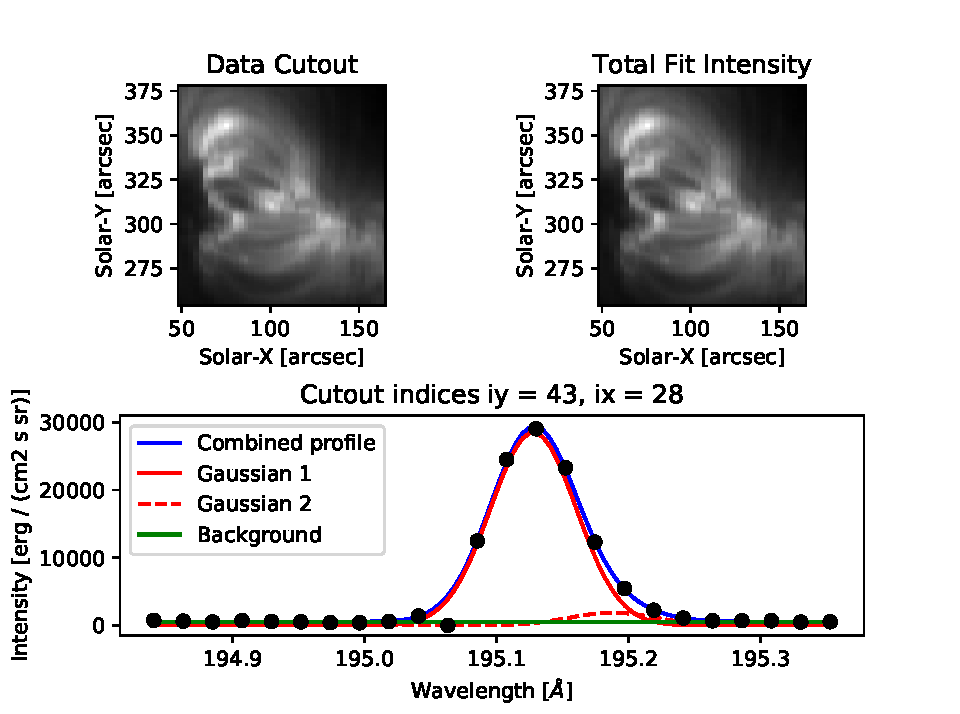
\includegraphics[clip,width=\linewidth]{figures/ex_cutout_and_fit.pdf}}
  \caption{Example data cutout and profile fits. The top two panels show the raster formed by summing
    over the wavelength axis on the observed intensities (left) and fit intensities (right).
    The bottom panel shows an example fit for the \ion{Fe}{12} 195.119\,\AA\ line profile.}
  \label{fig:fit_example}
\end{figure}